\documentclass{article}
\title{Blanchard Ch.13}
\author{Dawei Wang}
\date{\today}
\usepackage{ctex}
\usepackage{amsmath}
\usepackage{amssymb}
\usepackage{graphicx} %插入图片的宏包
\usepackage{float} %设置图片浮动位置的宏包
\usepackage{subfigure} %插入多图时用子图显示的宏包
\begin{document}
	\maketitle	

\section{短期的生产率、产出和失业}

把技术进步在生产函数中表示为技术水平A:

\[
Y=F(K,AN)
\]

忽略资本积累的作用,假设生产函数的形式为:

\[
Y=AN
\]

产出只由劳动力N来生产,单位工人生产A单位产出。A增加表示技术进步。

A在此处不仅代表技术水平,还代表人均生产水平(劳动生产率),由$ Y/N=A $得出。

因此就业为:

\[
N=Y/A
\]

短期内、产出水平是由IS和LM关系决定的。

\[
Y=Y(C-T)+I(r+x,Y)+G
\]

\[
r=\overline{r}
\]
	
提高生产率A的效果是什么,在实际政策利率不变的情况下,生产率提高是增加还是减少商品需求,答案是不确定的,因为生产率水平不会凭空提高,总需求的变动首先取决于是什么导致生产率提高。

假设是一项重要发明的普及使用使生产率提高,消费者对未来经济更乐观,增加消费。未来经济加快增长的预期,以及需要投入新技术,可能会导致投资骤增。这种情况下,对商品的需求增加;IS曲线向右移动,短期产出水平从Y增加到$ Y'' $。

\hspace*{\fill}

现在考虑生产率提高不是因为新技术的运用,而是因为现有技术高效运用的情况。这使很多企业不得不整顿生产,减少工作岗位。这些调整使生产率提高,与此同时总需求并没有增加:整顿生产几乎不需要新的投入。工人的不确定性增加,促使他们增加储蓄,减少消费。IS曲线左移,短期产出水平从Y下降到$ Y' $。

\begin{figure}[H] %H为当前位置,!htb为忽略美学标准,htbp为浮动图形
	\centering %图片居中
	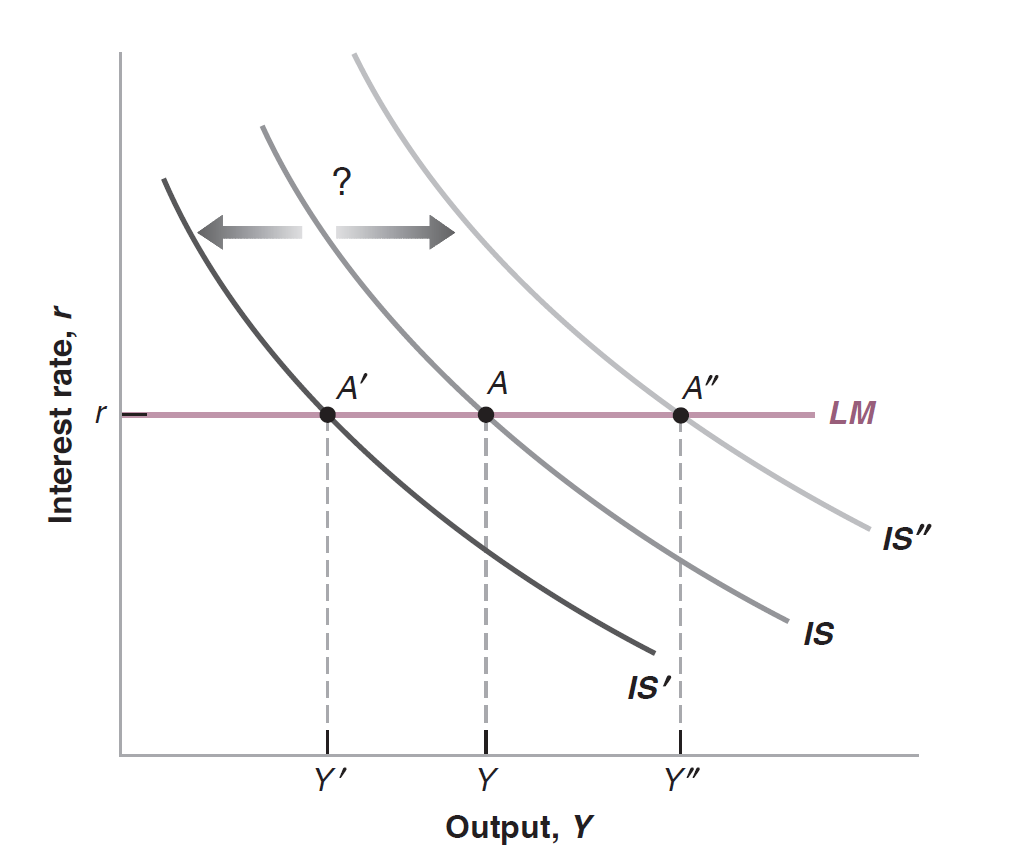
\includegraphics[width=1\textwidth]{13_1} %插入图片,[]中设置图片大小,{}中是图片文件名
	\caption{The Demand for Goods
		in the Short Run
		following an Increase in
		Productivity} %最终文档中希望显示的图片标题
	\label{Fig.main2} %用于文内引用的标签
\end{figure}

由式$ N=Y/A $:

就业变化的百分比=产出变化的百分比-生产率变化的百分比

因此产出增加的比例大于还是小于生产率的增加比例决定就业情况的变化。短期来说,生产率增加会导致失业增加或者减少,理论上得不出答案。

\section{生产率和自然失业率}

生产率变化会影响自然失业率吗?

技术性失业(technological unemployment):高失业率使是因为机器的使用,如果不对技术进步加以阻止的话,情况会更糟。、

然而简单地认为技术进步必然带来高失业率的观点显然是错误的。

在第七章中,我们认为自然失业率由两组关系决定:价格设定关系和工资设定关系。

\subsection{回顾价格设定和工资设定}

先考虑价格设定:

由式$ N=Y/A $,单位工人生产A单位产出,也就是说,生产1单位产出需要$ 1/A $个工人。

名义工资为W,则生产1单元产出的名义成本为$ (1/A)W=w/A $。

如果将价格设置为成本的1+m倍,m为加成,则价格为:

\[
P=(1+m)\frac{W}{A}
\]

考虑工资设定。有证据表明在其他条件不变的情况下,工资设定往往会反映生产率变化。拓展出工资设定公式:

\[
W=A^eP^eF(u,z)
\]

工人关心的是实际工资,而不是名义工资,因此工资取决于(预期的)价格水平$ P^e $。工资失业率取决于失业率u和其他因素z。

新的项$ A^e $:现在工资也取决于预期的生产率水平$ A^e $。如果工人和企业都预期生产率提高,那么在协定工资的时候会考虑这些预期。

\subsection{自然失业率}

假定对价格和生产率预期是正确的,即:$ P^e=P $,$ A^e=A $。

价格设定等式决定了企业的实际工资:

\[
\frac{W}{P}=\frac{A}{1+m}
\]

实际工资W/P与生产率水平A同比例增长:名义工资不变,生产率越高,企业制定的价格越低,则实际工资越高。

\begin{figure}[H] %H为当前位置,!htb为忽略美学标准,htbp为浮动图形
	\centering %图片居中
	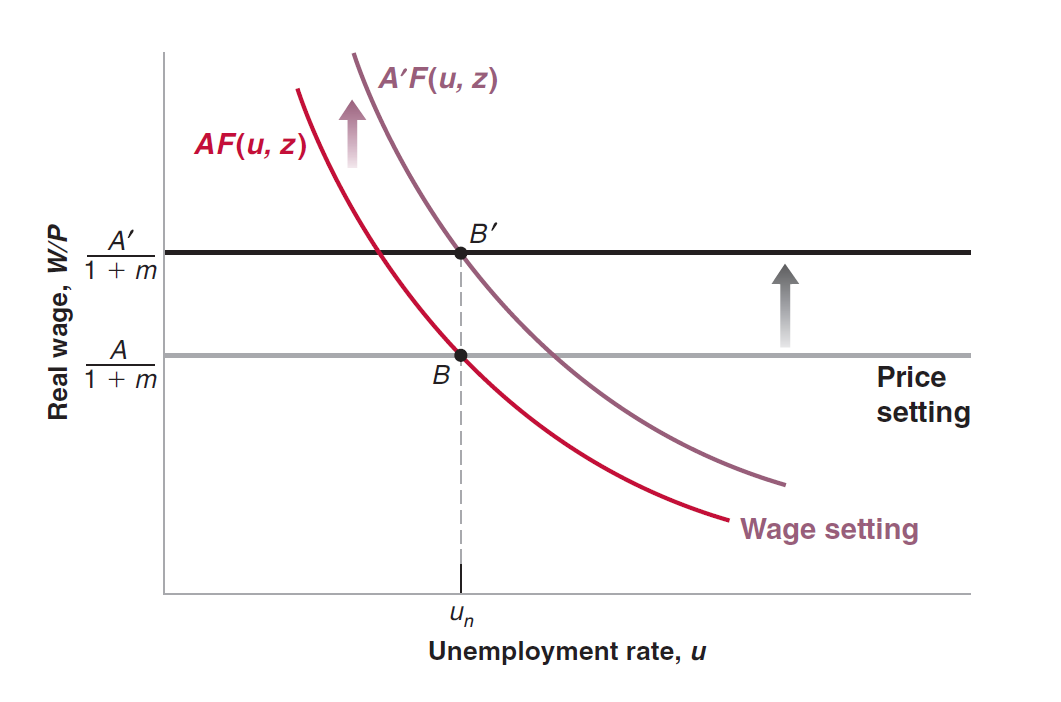
\includegraphics[width=1\textwidth]{13_2} %插入图片,[]中设置图片大小,{}中是图片文件名
	\caption{The Effects of an Increase
		in Productivity on
		the Natural Rate of
		Unemployment} %最终文档中希望显示的图片标题
	\label{Fig.main3} %用于文内引用的标签
\end{figure}

上图中的水平线表示:有价格决定的实际工资与失业率无关。

回到工资设定公式,在预期正确的前提下,$ P^e=P,A^e=A $,则工资设定公式为:

\[
\frac{W}{P}=AF(u,z)
\]

上图中向下倾斜的曲线表示:由工资设定得出的实际工资是失业率的递减函数。

在B点,劳动力市场均衡,自然失业率为$ u_n $。如果生产率水平变化,价格设定曲线向上移。失业率不变的情况下,由工资设定决定的实际工资也增长与价格设定决定的实际工资增长相同的水平。

因此在初始失业率$ u_n $处,两条曲线都上移同样的幅度。

得出来的结论很直观:工资不变,生产率提高3\%,价格会降低3\%,从而实际工资增加3\%。

自然失业率与生产率水平和生产率提高都无关。

\subsection{经验证据}

证据表明,需要很长一段时间才能将生产率预期调整到和现实一致的较低的生产率增长状况。当生产率因某个原因下降时,工人一般需要很长时间才能调整他们的预期。同时,工人不断地协商要求提高工资水平,而工资已经有被雨生产率较低的情况。

假设价格预期正确($ P^e=P $)而生产率预期并不一定与现实一致:

\[
\frac{W}{P}=\frac{A}{1+m}
\]

\[
\frac{W}{P}=A^eF(u,z)
\]

\begin{figure}[H] %H为当前位置,!htb为忽略美学标准,htbp为浮动图形
	\centering %图片居中
	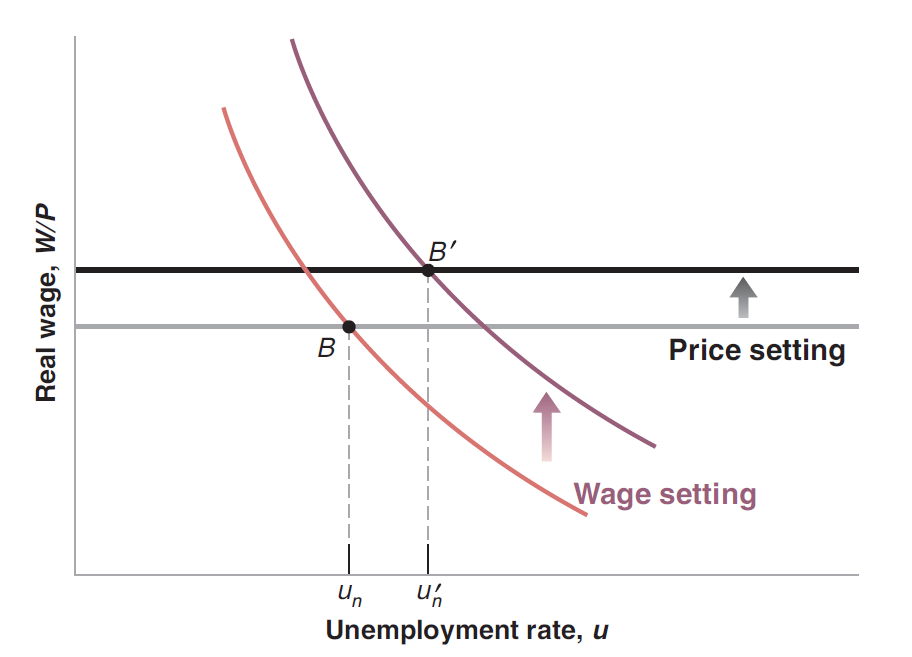
\includegraphics[width=1\textwidth]{13_3} %插入图片,[]中设置图片大小,{}中是图片文件名
	\caption{The Effects of a Decrease
		in Productivity Growth
		on the Unemployment
		Rate When Expectations
		of Productivity Growth
		Adjust Slowly} %最终文档中希望显示的图片标题
	\label{Fig.main4} %用于文内引用的标签
\end{figure}



假设生产率增长变缓:A的增长速度慢于从前,如果生产率增长预期调整缓慢,那么$ A^e $在一段时间内会大于A,工资设定曲线会比价格设定曲线移动得多,则自然失业率会从$ u_n $移动到$ u_n' $,自然失业率会保持在较高水平,直到生产率预期和现实一致,即$ A^e $再次和A相等。简而言之,生产率增长放缓后,工人要求的工资会高于企业能提供的工资水平,这就会使失业率上升,当工人最终调整预期的时候,自然失业率回到最初水平。

\hspace*{\fill}

总结:

短期来说,既没有理论也没有趋势得出生产率增长和失业率的系统性关系。

中期来说,即便生产率增长和失业率之间存在关系,也是反向关系。生产率增长放缓会使失业率增加,生产率提高会降低失业率。

对技术性失业的担忧可能来自于我们没有考虑技术进步的其他范畴,例如结构性变化(structural change),技术进步引起经济结构变化。对于一些工人来说,他们的技能被淘汰了,结构性变化对他们来说意味着失业或者低工资,或二者兼有之。

\section{技术进步、搅局和分配效应}

技术进步的过程实质上是创造性毁灭(creative destruction)的过程。新产品的出现使旧产品废弃,引入新技术需要新的技能,旧的技能不再适用。

\subsection{工资不平等加剧}

对于增长型部门或者有相应技巧的人来说,技术进步会带来新的机会和高工资,但对于衰退型部门和技巧被淘汰的人来说,技术进步可能意味着一段时间内的失业和低工资。

\subsection{工资不平等加剧的原因}

高技能工人的工资相对于低技能工人的工资增加的主要原因是对高技能工人的需求相对于低技能工人稳步增加。

为什么相对需求会稳定增加?

一种观点是因为国际贸易。该观点认为,雇佣大量低技能工人的美国企业被低工资国家的同类企业取代,被市场淘汰。同时为了保持竞争实力,企业将一部分生产转移到低成本国家。贸易和技术进步都有利于一国经济的发展,但都会带来结构性变化,使一些工人的境遇变糟。

另一种观点认为是因为技能型技术进步(skill-based technological progress)。新机器和新生产方法要求更多高技能工人。新生产方法要求工人更灵活,更好地适应新任务。灵活性则要求更多技能和教育。

不同于贸易派的解释的是,技能型技术进步能解释所有部门相对需求的变化。因此,大部分经济学家认为这是导致工资分配不均的主要原因。






















	
	
\end{document}